\documentclass[12pt]{article}
% Must be compiled by XeLaTeX
\def\CNBtitle{Manual\ for\ Using\ the\ cnbwp\ Class}
\usepackage{cnbwp-manual}
\setdefaultlanguage{english}
\title{Manual for Using the \fn{cnbwp} Class to Write CNB~Working~Papers}
\author{Zdeněk Wagner}\date{version 2013.12}
\begin{document}
\maketitle

\begin{abstract}\noindent This manual explains how to write Czech National Bank Working Papers
using the  \LaTeX typesetting system. The opening sections describe the \fn{cnbwp} class created
for this purpose. A separate section tells you how to prepare a list of references. The subsequent
sections give more generally applicable advice for creating and inserting figures and tables.
Section~\ref{publish} tells you the form in which the document has to be submitted and how the
document is edited. The names of the macros, packages, files and programs mentioned in this manual
are listed in the \hyperref[index]{index}. The manual also includes sample files, which are listed
in Section~\ref{vzor}. The class, the manual and the sample files were prepared for the Czech
National Bank. Martin Cincibuch from the CNB contributed significantly to the structure and content
of this document.  \end{abstract}

\tableofcontents

\section{Typographical Conventions}\label{typokon} Several font types with special meanings will be
used in this document. Text printed in \texttt{non-proportional font} will be used for printing out
pieces of code as they should be written in the source file in \LaTeX{}. This font may also appear
directly in the text in descriptions of macros. This means that \cmd{usepackage} and suchlike may
occur in the text. Names of parameters and other variable objects will be written in
\textit{italics}. In the section describing how to create a list of references we will use \bibi,
where \textit{typ} will substitute for part of the name of a macro. This will generally mean the
macros \cmd{bookItem}, \cmd{miscItem} etc.

For the names of files, packages and classes we will use \fn{sans-serif font}. Examples can be seen
in the document title and in the abstract. The exception to this will be URLs, where we need some
special characters. We will, therefore, print URLs in \texttt{non-proportional font} as well, e.g.
\zwurl{ftp://ftp.cstug.cz/pub/tex/CTAN/}, but this should not cause any confusion. We will also
write full file names with paths in the same way, e.g.
\zwurl{/usr/share/texmf-dist/tex/latex/cnb/cnbwp.cls}. These long names can be split across more
than one line without hyphenation.
	
Emphasised text will be printed in \textbf{bold font}, as italics are already being used for a
different purpose. Bold font is also used in the headings. In such cases, names of files, packages
and classes will be printed in \textbf{\fn{bold sans-serif font}}.

\pozor A large bold exclamation mark at the start of a paragraph indicates very important
information. Ignoring the instructions given in such a paragraph will cause a major error or an
error with a strange message (such that the cause of the error will be difficult to track down) to
occur during document preparation.

\section{Installation}\label{instalace}\index{installation} All macros used for writing CNB Working
Papers are implemented in the \fn{cnbwp.cls} class. The class is distributed in the archive file
\fn{cnbwp.zip}. The file is saved in the archive with a path conforming to the TDS~(\TeX\ Directory
Structure) standard. The installation method varies slightly depending on the specific \TeX{}
distribution.

\subsection{\MikTeX}\label{inst.miktex} Extract the \fn{cnbwp.zip} file to the \url{X:\localtexmf}
directory, where \texttt{X:} denotes the disk on which \MikTeX{} is installed
(usually~\texttt{C:}). Then open the menu \zwurl{Start/Programy/MikTeX/MikTeX Options}. On the
Roots tab, check that \url{X:\localtexmf} is on the list of directories searched. If not, add it.
Then click \texttt{Refresh FNDB}. To determine whether \LaTeX\ will locate the class, use
the command:

\begin{verbatim}
findtexmf cnbwp.cls
\end{verbatim}

\noindent If everything is OK, the command will print the full path for the \fn{cnbwp.cls}
file.

\pozor The \url{X:\localtexmf} directory is intended for local files that are not a
standard
component of \MikTeX. If you update \MikTeX\, this directory will not be overwritten, so
you will
not lose the files.

\subsection{\teTeX}\label{inst.tetex} This distribution is the standard in Unix systems
and is also
available for OS/2 and eComStation. We will describe the installation in Linux only. The
installation in OS/2 is similar, differing only in that a backslash is used to separate
the
directories and the name of the disk on which \teTeX\ has been installed must be entered
explicitly.

Extract the \fn{cnbwp.zip} file to the \url{/usr/share/texmf-local} directory. When
installing in
Unix systems, you must make sure that the
\url{/usr/share/texmf-local/tex/latex/cnb/cnbwp.cls} file
does not have DOS line ends. Once the file has been extracted, the file database usually
needs to
be refreshed using the \texttt{mktexlsr} command.

\TeXLive\ is based on this distribution, so everything described in the following
section applies to \teTeX\ as well.

\subsection{\TeXLive}\label{inst.tl} \TeXLive\ is a popular multiplatform \TeX{} distribution. It
comes from the same sources as \hyperref[inst.tetex]{\teTeX}, so the installation is similar. The
directory to which \fn{cnbwp.zip} should be extracted is usually
\url{/usr/local/texlive/texmf-local} in Unix
systems and \url{X:\TeXLive\texmf-local} in Windows. However, \TeXLive\ may be installed
in any
directory and you can even have several versions of \TeXLive\ installed simultaneously.
The
directory to which \fn{cnbwp.zip} should be extracted can be determined using the command:

\begin{verbatim}
kpsewhich --expand-var=$TEXMFLOCAL
\end{verbatim}
\index{kpsewhich}

The \texttt{texmf-local} directory tree is shared by all \TeXLive\ versions installed on
a computer. If a newer version is installed, the files will automatically be found.

\pozor The \TeXLive\ distribution usually requires \texttt{mktexlsr} to be run after the files have
been added. In distributions for Windows there is even an item in the \TeXLive menu for this
purpose. If the database is not refreshed using \texttt{mktexlsr} and two exclamation marks are
given in front of the name of the directory containing the \fn{cnbwp} class, \LaTeX\ will not be
able to locate the class. To determine whether \LaTeX\ will locate the class, use the command:

\begin{verbatim}
kpsewhich cnbwp.cls -progname latex
\end{verbatim}	

\noindent If everything is OK, the command will print the full path for the \fn{cnbwp.cls} file.

\subsection{\emTeX}\label{inst.emtex} This distribution is obsolete and Eberhard Mattes no longer
maintains it. It is better to switch to another distribution. However, if you do want to use
\emTeX, extract \fn{cnbwp.zip} to an auxiliary directory, create a \fn{cnb} subdirectory
in
\url{X:\emtex\texinput\latex2e} and copy \fn{cnbwp.cls} and \fn{cnbwpsizes.clo} into it.

\subsection{Scientific Word}\label{inst.sciword} This manual is written for version 5.5. In this
version, extract \fn{cnbwp.zip} to \url{X:\sw55\TCITeX}. In other versions the name of the root
directory will probably differ. Scientific Word does not adhere strictly to TDS, as the directory
names contain both lower-case and upper-case letters. However, the FAT and NTFS file systems are
not case sensitive, so this should not cause any problems.
	
\subsection{Other Distributions}\label{inst.other} To install the \fn{cnbwp} class in other
distributions you will need to follow the instructions given in the manual supplied with the
relevant distribution. The current distributions are usually based on \fn{web2c} and conform to the
TDS standard, so the installation procedure is analogous to that for \hyperref[inst.tl]{\TeXLive,
see section~\ref*{inst.tl}}.

\subsection{Preparing Documents from Scientific Word in Other
Distributions}\label{sciword.elsewhere} Documents created using Scientific Word require specific
macros defined in files in the \fn{SWmacros} directory. These files are freely distributable. So if
you want to process a document in another distribution, copy the entire directory to
\url{texmf-local/tex/latex} or \url{localtexmf/tex/latex}, depending on which distribution you are
using.

\pozor Remember that in some distributions after adding files you have to refresh the database
either using the \texttt{mktexlsr} command or from the menu.

\section{Testing the Installation}\label{test.inst} In many distributions the installation can be
tested using the \texttt{kpsewhich} command, as mentioned in section~\ref{inst.tl}. This enables
you to check whether \LaTeX\ is able to locate the \fn{cnbwp} class and the macros from the
\fn{SWmacros} directory. If you do not have \texttt{kpsewhich} in your distribution, all you need
to do is write a simple document:

\begin{verbatim}
\documentclass{cnbwp}
\begin{document}
Hello world.
\end{document}
\end{verbatim}

\noindent
If, when processing this document, \LaTeX\ returns with:

\begin{verbatim}
! LaTeX error: file `cnbwp.cls' not found
\end{verbatim}

\noindent the class is not installed correctly. In this event, check whether you followed the
instructions given in the relevant section correctly.

\section{Document Structure}\label{struktura} A working paper is a standard document written in
\LaTeX{} and thus consists of the standard parts: a preamble and a document body. Everything
preceding the command \cmd{begin\{document\}} is part of the preamble. The list of references is a
special part of the document body and is dealt with separately in
\hyperref[references]{section~\ref*{references}}.

\subsection{Preamble}\label{preambule}\index{preamble}
All the main macros are implemented in the \fn{cnbwp} class. Each document must therefore start with the command:

\begin{verbatim}
\documentclass{cnbwp}
\end{verbatim}

The \xx\cmd{documentclass} command allows parameters to be entered in square brackets before the
class name. This case is no exception. \fn{cnbwp} is derived from the \fn{article} class and
assumes all its parameters. The Working Papers format is a fixed one, however, so parameters that
alter the paper size, the font size, and number of columns are ignored.

A number of new parameters may be used in the \fn{cnbwp} class. The first of these concerns the
numbering of figures and tables. By default, tables and figures are numbered
nonhierarchically. The numbering mode can be changed. It is set using
the following parameters:

\vb\noindent
\begin{tabular}{@{}Rl}
hierarchicalnumbering & hierarchical numbering \\
simplenumbering & simple numbering
\end{tabular}\label{numbering}\index{hierarchicalnumbering}\index{simplenumbering}\vb

If neither of these parameters is specified, or if both are specified, simple numbering
will
be used. Hierarchical numbering can be activated with the command:

\begin{verbatim}
\documentclass[hierarchicalnumbering]{cnbwp}
\end{verbatim}

Figure and table captions are left-aligned by default. In some documents it may look better
aesthetically if the captions are centred. The alignment for the document as a whole is set using
the following parameters:

\vb\noindent
\begin{tabular}{@{}Rl}
standardcaptions & captions left-aligned \\
centeredcaptions & captions centred
\end{tabular}\label{captions}\index{standardcaptions}\index{centeredcaptions}\vb

If neither of these parameters is specified, or if both are specified, the figure and table
captions will be left-aligned.

In some circumstances it is necessary to align some captions differently than other captions in the
document. This can be done using macros that will be explained later on in section~\ref{body}.
	
The \fn{cnbwp} class implicitly loads the packages needed for formatting Working Papers. These
packages are: \xx\fn{ifpdf}, \fn{mathptmx}, \fn{fontenc} with T1 parameter, \fn{babel}
with czech and english parameters, \xx\fn{natbib}, \xx\fn{url} and \xx\fn{keyval}. The
parameters
specified in square brackets in the \xx\cmd{documentclass} command are automatically sent to all
these packages as well as to any other packages that you might load later on. You will probably
most often specify parameters for the \fn{natbib} package. If you wish to change the citation style
from author-year to numbered format, use:

\begin{verbatim}
\documentclass[numbered]{cnbwp}
\end{verbatim}
\index{numbered}

The parameters can be used in any combination you like. It does not matter which order you list
them in. If, then, you want a base font size of 10.95\,pt, centred captions and numbered literature
references, you can write:

\begin{verbatim}
\documentclass[centeredcaptions,numbered,11pt]{cnbwp}
\end{verbatim}

Using the \xx\cmd{usepackage} command you can now load the other packages you need to format your
document. In a single \cmd{usepackage} command you can specify two or more packages separated by
commas, e.g.:

\begin{verbatim}
\usepackage{graphicx,amsmath,dcolumn}
\end{verbatim}

The \cmd{usepackage} macro also lets you specify parameters in square brackets. These parameters
are only sent to the packages specified in the given command. However, you cannot then load more
than one package using the same command, as \LaTeX\ would display a message stating that the
parameters are not implemented in the package. You need to use, for instance:

\begin{verbatim}
\usepackage{amsmath,dcolumn}
\usepackage[dvips]{graphicx}
\usepackage[figuresright]{rotating}
\end{verbatim}

The parameters specified in the \xx\cmd{documentclass} command will be sent to all packages. Thus
the parameter \texttt{draft} can be specified globally:

\begin{verbatim}
\documentclass[draft]{cnbwp}
\usepackage{graphicx}
\end{verbatim}

\noindent
However, you can also use it with the \fn{graphicx} package only:

\begin{verbatim}
\documentclass{cnbwp}
\usepackage[draft]{graphicx}
\end{verbatim}

\noindent In both cases the figures will be replaced by a rectangular box of the same size as the
figure and the file name will be printed inside this box. In the first case, moreover, overfull
boxes will be indicated by black rectangles in the margin.

\pozor The \xx\fn{hyperref} package uses a different definition of the \xx\cmd{url} macro than the
\xx\fn{url} package. In addition, this definition causes conflicts in the bibliography. The
\fn{cnbwp} class therefore copies the \cmd{url} definition from the \fn{url} package to an
auxiliary macro \cmd{CNBurl}, and after \cmd{begin\{document\}} is executed the \cmd{url} macro
definition is refreshed so that it corresponds to the \fn{url} package. If you wish to use the
macro from the \fn{hyperref} package, save it after loading the package in a macro with a suitable
name, e.g. using:

\begin{verbatim}
\let\MYurl\url
\end{verbatim}

\pozor Never change the \cmd{url} macro definition, as the macros for formatting the list of
references depend on this definition. The \cmd{url} macro may be used in the citation database
drawn up by \BibTeX, so you will not necessarily see it directly in the document. If the definition
is changed, \LaTeX\ will display strange error messages and the formatting of part of the document
will probably crash completely.

\pozor \LaTeX\ does not require the use of separate name files for each package. Packages may
therefore contain conflicting definitions that can cause unpredictable errors. Besides the
conflicts mentioned above, the \xx\fn{path} package cannot be used at the same time as the
\xx\fn{url} package. It is therefore a good idea to begin with a minimal document and only use
those packages which are absolutely necessary for processing. Conflicts have to be located and
eliminated by trial and error. Sometimes it also helps to change the order in which you load the
packages.

At the end of the preamble you should define your own macros needed throughout the document. The
\xx\cmd{DeclareRobustCommand} command is especially useful for defining macros. It has the same
syntax as \xx\cmd{newcommand}. The only difference is that the defined macro is robust. When using
macros defined in this way in the \cmd{section} and \cmd{subsection} commands, you do not need to
use \xx\cmd{protect}.

In some cases you will need to adjust the margin settings, as some printer drivers ignore the
margins set in the file and move the text. Before you start making changes, check your printer's
properties. Some drivers always default to letter format, which means that you have to change the
format to A4 before each print job. If the margins still disagree, make adjustments in the
registers \xx\cmd{hoffset} (to move the text horizontally) and \xx\cmd{voffset} (to move the text
vertically). For instance, if you need to move the text 5\,mm to the right and 3\,mm upwards,
write:

\begin{verbatim}
\hoffset=5mm
\voffset=-3mm
\end{verbatim}

You can ascertain the values by printing out a test figure in \xx\fn{a4-portrait.pdf}.

\subsection{Title Page}\label{titlepage} A Working Paper must always start with a title page, which
is made up of several components. The following subsections will deal with each of these in turn.

\subsubsection{Title}\label{nadpis} The title lies at the boundary between the preamble and the
document body. In fact, some macros can be put in the preamble. More precisely, the macros defining
the title, the names of the authors and the acknowledgements can be written anywhere
between \cmd{documentclass} and
\cmd{maketitle}. It can thus be useful to place them right at the beginning of the file.

The title of the work is written as the argument of the \xx\cmd{title} macro. The title
will be
printed later, after you write the \xx\cmd{maketitle} command, but it will also be put in
the
header:

\begin{verbatim}
\title{Twelfth Night, or What You Will}
\end{verbatim}


The names of the authors are entered using the \xx\cmd{author} macro that requires two
parameters. The first parameter conains the full name. The authors' institution is
entered in the second argument , e.g. as follows:

\begin{verbatim}
\author{Captain Nemo}{Nautilus}
\author{Robinson Crusoe}{Desert Island}
\end{verbatim}

\subsubsection{Acknowledgements}\label{ack} Acknowledgements are an optional part of a
Working
Paper. They are written in the argument of the \xx\cmd{acknowledge} macro.

The title will be printed by specifying the \xx\cmd{maketitle} macro. This macro must
come after \cmd{begin\{document\}}.

\subsubsection{Abstract}\label{abstrakt}
The English abstract should be placed in the \xx\texttt{abstract} environment, the Czech
abstract should appear in the \xx\texttt{abstrakt} environment, i.e. as follows:

\begin{verbatim}
\begin{abstract}
Place the abstract here.

The abstract may contain more than one paragraph. A blank line should be left
between the paragraphs. No blank line is needed at the end of the abstract.
\end{abstract}

\begin{abstrakt}
Zde uvedeme abstrakt práce.

Abstrakt může obsahovat více odstavců. Mezi odstavci ponecháme
prázdný řádek. Na konci abstraktu prázdný řádek být nemusí.
\end{abstrakt}
\end{verbatim}

Czech hyphenation rules are activated automatically in the \texttt{abstrakt} environment.

\subsubsection{JEL Codes}\label{jel}
JEL codes should be put in the \xx\cmd{JEL} macro:

\begin{verbatim}
\JEL{E22, E23, E32, E52}
\end{verbatim}

\subsubsection{Keywords}\label{kwd}
Keywords are the final element of the title page. They are entered using the aforementioned \xx\cmd{Keywords} macro:

\begin{verbatim}
\Keywords{20,000 leagues, maelstrom, Nautilus, sea, whale}
\end{verbatim}

The CNB requires keywords to be given in alphabetical order. However, the above macro does not
perform this task, so authors must do it themselves.
	
\subsection{Nontechnical Summary}\label{nontech} The Nontechnical Summary is about one page long
and is printed on a separate page in the document. Like the abstract, it is written in the
\xx\texttt{nontechsummary} environment:

\begin{verbatim}
\begin{nontechsummary}
Write the Nontechnical Summary in this environment. The title will be
created automatically and will not be numbered.

The text usually consists of several paragraphs separated by blank lines.
\end{nontechsummary}
\end{verbatim}

\pozor The \hyperref[kwd]{\xx\cmd{Keywords}} macro and the \xx\texttt{nontechsummary} environment
force a page break. If both these elements
are missing and the page break is forced manually using the \cmd{newpage} or \cmd{clearpage}
command, part of the document will be incorrectly formatted.

\subsection{Macros for the Document Body }\label{body} The body of the document is written in the
same way as with the \fn{article} class. Sections are therefore specified using the
\xx\cmd{section} macro and subsections using the \xx\cmd{subsection} macro. The
\xx\cmd{subsubsection} command is also implemented. Subdivision to \xx\cmd{paragraph} and
\xx\cmd{subparagraph} was not envisaged in the design, but no syntax error will occur if these
macros are used.

Table and figure captions are written in the \xx\cmd{caption} macro. The captions will be aligned
according to the parameter specified in the preamble (see
\hyperref[captions]{page~\pageref*{captions}}). If you wish to align a caption
differently, you
must explicitly specify \xx\cmd{standardcaption} to left-align it and
\xx\cmd{centeredcaption} to
centre it. The numbering format always corresponds to the parameters specified in the
preamble,
which are explained \hyperref[numbering]{on page~\pageref*{numbering}}. It cannot be
changed in the
document. This would be nonsensical from the typographical perspective anyway.

The description of a table or a figure may contain a note entered by using the
\xx\cmd{Note} macro and information on a source entered by using a \xx\cmd{Source} macro.
They are usually placed below the \xx\cmd{caption} macro as follows:

\begin{verbatim}
\Note{Value Added Tax (VAT), Excises (E), Personal Income Tax (PIT),
      Social Security Contributions (SSC), Inheritance Tax (IT),
      Corporate Income Tax (CIT), Other Age-Specific Revenues (OR).}
\Source{CNB}
\end{verbatim}

\section{References}\label{references} The list of references (bibliography) can be
written in two
ways: either using the \BibTeX{} system, or not using it. In either case the
\xx\fn{natbib}
package, which is automatically loaded by \fn{cnbwp}, is used for the actual formatting.
Consequently, the appearance of the document does not depend on the method chosen for
writing the
list of references.

Parameters can be transferred to the \xx\fn{natbib} package as follows. Optional
parameters can be
written in square brackets in the \cmd{documentclass} command. These parameters are sent
both to
the \fn{article} class, from which the \fn{cnbwp} is derived, and to all the loaded
packages. Thus
it is possible to specify parameters for the \xx\fn{natbib} package. For example, the
citation
style can be changed from author-year to numbered format using the \xx\texttt{numbered}
parameter.

The method for creating a list of references using \BibTeX{} will be described briefly in
section~\ref{bibtex}. The macros created for Czech National Bank Working Papers will be
explained
in detail in section~\ref{makra} and the subsections thereof.

\subsection{Writing References Using \BibTeX{}}\label{bibtex}\index{BibTeX@\BibTeX} The
use of
\BibTeX{} is described in Oren Patashnik's document \uv{\BibTeX ing}, which comes as part
of the
standard \TeX{} distributions. We will make use of the \xx\fn{abbrvcnb} style derived
from the \xx\fn{natbib} bibliographic
styles. Let's assume that you have a bibliography database stored in a file called
\fn{references.bib}. You should then place the following in the \LaTeX document:

\begin{verbatim}
\bibliographystyle{abbrvcnb}
\bibliography{references}
\end{verbatim}
\index{abbrvnat}\index{bibliography@\cmd {bibliography}}\index{bibliographystyle@\cmd
{bibliographystyle}}

\noindent
Once the document has been processed by \LaTeX{}, run \BibTeX:

\begin{verbatim}
bibtex document
\end{verbatim}

\noindent (In place of the word \textit{document} write the file name; here we have assumed that
the document is stored in a file called \fn{document.tex}.) The document then needs to be processed
twice by \LaTeX{}. Occasionally a third pass is required if a page shift occurs after the
references are added to the text.

Document URLs are usually long strings in which automatic hyphenation does not work or the words
are hyphenated in inappropriate places, hence confusion can arise. This problem is solved in
conformity with the standards for writing URLs\index{URLs} in the \xx\fn{url} package, which is
also implicitly loaded by the \fn{cnbwp} class. The URL usually appears in a
\textit{note}\index{note} field. This field should therefore be written as follows:

\begin{verbatim}
note = "\url{ftp://ftp.cstug.cz/pub/tex/CTAN/}",
\end{verbatim}
\index{url@\cmd  {url}}

\subsection{Writing References Using Special Macros}\label{makra} The list of references can be
written using special macros directly in the \LaTeX file in the \xx\texttt{thebibliography}
environment. This environment has one required parameter, which sets the width needed for the
ordinal. \BibTeX{} enters the number of the citations in this parameter. You may, however, specify
any text of suitable width, for instance \texttt{XX}, as used in the example (see the
\hyperref[priloha]{Appendix}). Each citation is written in the following format:

\medskip\noindent
\bibi\texttt{[}\textit{citation text}\texttt{]}\texttt{\{}\textit{label}\texttt{\}}%
\texttt{\{}\textit{citation content}\texttt{\}}

\medskip\noindent In place of the word \textit{type} you need to specify the relevant type of work
cited. We will use an identifier derived from the standard types defined in \BibTeX{}. A list and
description of these can be found in \hyperref[typy]{section~\ref*{typy}}.

The first two parameters (optional and required) have the same meaning as for the \xx\cmd{bibitem}
macro. The required parameter \textit{label} is used when citing text in the \xx\cmd{cite} macro.
The optional parameter \textit{citation text} contains the information that is written in the text
at the citation location. This parameter has the general format:

\medskip\noindent
\texttt{[}\textit{short text}\texttt{(}\textit{year}\texttt{)}\textit{long text}\texttt{]}

\medskip \pozor The final parameter of \bibi\ macros is processed using the \xx\fn{keyval} package.
This means that only declared fields may be used. It is not possible to create an unknown field to
add a comment that is not meant to be printed. Such an attempt will lead to an error during the
processing of the document. Comments are written after a \textit{procento} sign, as in standard
\LaTeX texts.

The optional parameter and the first required parameter of \bibi\ macros are transferred unchanged
to the \xx\cmd{bibitem} macro.
	
The \fn{natbib} package can choose between short and long text. If the cited work has only one
author, \textit{dlouhý text} is not specified. The entire parameter can then be written in the
following format:
	
\begin{verbatim}
[Mouse(1984)]
\end{verbatim}

Both options are specified for works with more than one author. If, for example, you want to cite a
book issued in 1984 written by Mickey Mouse, Donald Duck and Bugs Bunny, the parameter should be
written in the following format:

\begin{verbatim}
[Mouse et.~al.(1984)Mouse, Duck and Bunny]
\end{verbatim}

\pozor
\BibTeX\ generates all pieces of information for the \bibi\ macro automatically. If the
information is entered manually, the parameter in the square brackets must be properly
formatted. Especially, the value in the round parentheses must be identical to the
\texttt{year} value as shown in appendix~\ref{priloha}. The items must also be sorted by
the author.

Selection of the citation text format is based on the required appearance of the resulting text. If
you do not require citations in long format, you need not specify that option in the \bibi\ macro.

The \xx\fn{natbib} package requires round brackets in the optional parameter. If you do not know
the year of publication of a cited work, you must write at least empty brackets~\texttt{()}.

The reference to the cited work is written in \textit{citation content}. The format of this
parameter will be described in \hyperref[obsah]{section~\ref*{obsah}}.

\subsubsection{Types of Cited Works}\label{typy} The macros used for citing works are based on the
standard types defined in \BibTeX{}. Here we will list and briefly describe these types and provide
a list of the required and optional fields. The meaning of the fields and the way they are written
will be explained in \hyperref[obsah]{the following section}.

\begin{description}
\item[\xx\cmd{articleItem}] An article from a journal or magazine. Required fields: \;author , \;title , \;journal ,
\;year . Optional fields: \;volume , \;number , \;pages , \;month , \;note .

\item[\xx\cmd{bookItem}] A book with an explicit publisher. Required fields: \;author \ or \;editor ,
\;title , \;publisher , \;year . Optional fields: \;volume \ or \;number , \;series , \;address
, \;edition , \;month , \;note .

\item[\xx\cmd{bookletItem}] A work that is printed and bound, but without a named publisher or institution.
Required field: \;title . Optional fields: \;author , \;howpublished , \;address , \;edition ,
\;month , \;year , \;note .

\item[\xx\cmd{conferenceItem}] The same as \xx\cmd{inproceedingsItem}.

\item[\xx\cmd{inbookItem}] A part of a book, usually a chapter or a range of pages. Required
fields: \;author \ or \;editor , \;title , \;chapter \ and/or \;pages , \;publisher , \;year .
Optional fields: \;volume \ or \;number , \;series , \;type , \;address , \;edition , \;month ,
\;note .  The meaning of the \;type \ field will be explained \hyperref[type]{on
page~\pageref*{type}}.

\item[\xx\cmd{incollectionItem}] A part of a book having its own title. Required fields: \;author ,
\;title
, \;booktitle , \;publisher , \;year . Optional fields: \;editor , \;volume \ or \;number ,
\;series , \;type , \;chapter , \;pages , \;address , \;edition , \;month , \;note .
The \;type \ field has the same meaning as in the previous citation type and is explained \hyperref[type]{on page~\pageref*{type}}.

\item[\xx\cmd{inproceedingsItem}] An article in a conference proceedings. Required fields: \;author ,
\;title ,
\;booktitle , \;year . Optional fields: \;editor , \;volume \ or \;number , \;series , \;pages ,
\;address , \;edition , \;month , \;organization , \;publisher , \;note .

\item[\xx\cmd{manualItem}] Technical documentation. Required field: \;title . Optional fields:
\;author , \;organization , \;address , \;edition , \;month , \;year , \;note .

\item[\xx\cmd{mastersthesisItem}] A Master's thesis. Required fields: \;author , \;title , \;school ,
\;year . Optional fields: \;type , \;address , \;month , \;note .


\item[\xx\cmd{miscItem}] Another type used when nothing else fits. It has optional fields only
\;author , \;title , \;howpublished , \;month , \;year , \;note .

\item[\xx\cmd{phdthesisItem}] A PhD thesis. Required fields: \;author , \;title , \;school ,
\;year . Optional fields: \;type , \;address , \;month , \;note .

\item[\xx\cmd{proceedingsItem}] The proceedings of a conference. Required fields: \;title , \;year
. Optional fields: \;editor , \;volume \ or \;number , \;series , \;address , \;month ,
\;organization , \;publisher , \;note .

\item[\xx\cmd{techreportItem}] A report published by a school or other institution, usually
numbered within a series. Required fields: \;author , \;title , \;institution , \;year . Optional
fields: \;type , \;number , \;address , \;month , \;note .

\item[\xx\cmd{unpublishedItem}] A document having an author and title, but not formally published.
Required fields: \;author , \;title , \;note . Optional fields: \;month , \;year .

If none of these types meets your requirements, you can use \xx\cmd{bibitem} directly and format everything manually.

\end{description}


\subsubsection{Specifying Fields}\label{obsah}
The content of each field of a cited work is entered in the last parameter of \bibi\ macros. The fields are specified in the following format:

\begin{verbatim}
{name1 = value1, name2 = value2, name3 = value3}
\end{verbatim}

\noindent Spaces around equals signs and commas separating fields are ignored. Blank fields are
also ignored. It is therefore possible to write two or more commas in succession or a comma before
the first field and after the last one. Wherever a space is permitted, a line can also be
terminated. In addition, \TeX{} ignores all spaces at the start of a line. The list of references
can thus be written in a clear, easy-to-read style like that used in the
\hyperref[priloha]{Appendix}.

Fields are separated from one another with commas. If you want to write a comma in the field value,
you have to enclose the entire value in curly brackets. This will occur most frequently in
citations of works with more than one author. Where a publication has only two authors, their names
should be joined with the conjunction \textit{and} as follows:

\begin{verbatim}
author = Donald Duck and Mickey Mouse, ...
\end{verbatim}

\noindent
Here a comma terminates the field. If there are more authors, their names should be enclosed in brackets as follows:

\begin{verbatim}
author = {Donald Duck, Mickey Mouse, and Bugs Bunny}, ...
\end{verbatim}

\noindent
The first comma (inside the brackets) is part of the list of authors, and the last comma
terminates the field. In case of three or more authors the conjunction \textit{and}
should be preceded by a comma.

\pozor Omitting a comma or leaving out the brackets around a value containing a comma
results in an
error message about an unknown field with a strange name. Sometimes errors of this type
cause the
loss of an entire chunk of the list of references and subsequent parts of the document.

Curly brackets are often used in database files destined for processing by \BibTeX{} in
order to
prevent conversion to upper-case or lower-case letters. \LaTeX\ does not perform any
conversions,
so brackets are not needed. However, various macros can be used, e.g. \xx\cmd{mbox} to
prevent
incorrect hyphenation and \xx\cmd{-} to specify where to hyphenate words correctly, and
inside the
\xx\texttt{thebibliography} environment you can even define your own macros, which will be
unknown
(or defined differently) in other parts of the document.

Fields can be entered in any order, but only the following may be used:

\begin{description}
\xitem[address] The address of the publisher or institution (e.g. the school in the case
of a thesis)
\xitem[author] The name(s) of the author(s), in the format as they should appear. Unlike
\BibTeX{}
there is no reformatting (forenames will not be shortened to initials etc.).
\xitem[booktitle] Title of a book, part of which is being cited.
\xitem[chapter] A chapter number.
\xitem[edition] The edition. This should be an ordinal and can also be entered as a word,
e.g. \textit{Second}.
\xitem[editor] Name(s) of editor(s), entered in the same format as the author names.
\xitem[howpublished] How something strange has been published.
\xitem[institution] The sponsoring institution of a technical report
(\cmd{techreportItem}).
\xitem[journal] A journal name or abbreviation.
\xitem[month] The month in which the work was published. The day can also be given in this
field.
\xitem[note] An explanatory note. This field is given in the examples in the
\hyperref[priloha]{Appendix}, but it is rarely used in practice. It is used to state the
URLs\index{URLs} of works published on the Internet. For automatic and correct splitting
of long
URLs on multiple lines, the \xx\fn{url} package loaded by the \fn{cnbwp} class is used.
URLs should
therefore be written in the following format:

\begin{verbatim}
note = \url{ftp://ftp.cstug.cz/pub/tex/CTAN/}, ...
\end{verbatim}

\xitem[number] The number of a journal, magazine, technical report, or of a work in a
series.
\xitem[organization] The organisation that sponsors a conference or that publishes a
manual.
\xitem[pages] A range of pages.
\xitem[publisher] The publisher's name.
\xitem[school] The name of the school where a thesis was written.
\xitem[series] The name of a series (or set) of books.
\xitem[title] The work's title.
\xitem[type] The type of a work\label{type}, e.g. \textit{Research Note}. In citations
\xx\cmd{inbookItem} and \xx\cmd{incollectionItem} specify the text corresponding to the
\;chapter
\index{chapter} field. The default is \texttt{chapter}, but you can specify
\texttt{section}, for
example.
\xitem[volume] The volume of a journal or multi-volume book.
\xitem[year] The year of publication or, for an unpublished work, the year it was written.
\end{description}

The breakdown into fields need not be strictly observed. The information can be split into
separate
fields:

\begin{verbatim}
publisher = John Wiley \& Sons, address = New York, ...
\end{verbatim}

The list of references written directly in a \LaTeX document will probably not be used for
further
machine processing. It may therefore be useful to combine the two pieces of information
into a
single field:
	
\begin{verbatim}
publisher = {John Wiley \& Sons, New York}, ...
\end{verbatim}

\noindent Here we had to use brackets, as the combined information contains a comma.

Macros automatically add full stops or commas as individual fields, although only where
the text
does not end in a punctuation mark. Consider a title typed as:

\begin{verbatim}
title = Can we spend less money for more music?, ...
\end{verbatim}

\noindent In this case no punctuation mark will be added, even if the entire title is
enclosed in
curly brackets.

\subsection{How to Choose the Entry Type} An entry type must be chosen for making \BibTeX
database
entries and when using \bibi\ macros. The type names are intuitive and it should be
straightforward
to make the right choice. In cases of doubt, it helps to know which fields are required
and which
are optional. Choose the type whose structure best fits the purpose.

Some fields seem superfluous. For example, the bibliographic types for Master's
(\xx\cmd{mastersthesisItem}) and Ph.\,D.
(\xx\cmd{phdthesisItem})\footnote{In \BibTeX{} \xx\texttt{@mastersthesis} and
\xx\texttt{@phdthesis}.} thesis have exactly the same format. The only difference is the
default value of
the optional field \;type . If you want to cite a similar publication, for instance a
dissertation,
you can use any type and specify the optional field:

\begin{verbatim}
type = Dissertation, ...
\end{verbatim}

Works only available from the Internet have not been formally published. For such
publications, use
\xx\cmd{unpublishedItem} (in \xx\BibTeX{} \texttt{@unpublished}). URLs of works should be
placed in
the \;note \index{note} field, as mentioned earlier.

%\subsection{Technická poznámka}
% Technickou poznamku navrhuji rozdelit a presunout jak navrzeno


\section{Figures and Charts}\label{incgraph} \TeX\ is a text-processing program. Apart
from
primitive graphics created with horizontal and vertical strokes and characters made from
specially
prepared fonts, no figures can be created directly. You can, however,
import\footnote{Technical
speaking, there isn't even a command for inserting figures. However, \TeX\ does have the
\xx\cmd{special} command, which is not interpreted at all and whose argument is merely
sent to the
output device. How this command is handled depends on the relevant driver. When we talk
about how
figures are inserted in \TeX or \LaTeX documents, we are always referring to some specific
device
driver.} figures created in other applications and saved in separate files.

Figure and tables can be (but do not have to be) inserted in the text using the floating
environments \xx\texttt{figure} and \xx\texttt{table}, which among other things allow such
objects
to be easily numbered, described, placed and, as the case may be, further manipulated. For
a
description of some of the more advanced techniques for working with floating
environments, see
also section \ref{plovouci}.

The easiest way to load a figure into a floating environment is to use the
\xx\fn{graphicx}
package. The \xx\cmd{includegraphics} macro has one required parameter -- the name of the
file
containing the figure. A series of different instructions can be specified in the optional
parameter in square brackets in the format \textit{key=value}. The syntax is the same as
for the
\bibi\ macro, which was described in section~\ref{obsah}, except that square brackets are
used
instead of curly brackets, as the first parameter is optional. Here, too, the parameters
are
processed using the \xx\fn{keyval} package.

A detailed description of the \cmd{includegraphics} command can be found in the file
\xx\fn{grfguide.ps}, which is part of the distribution. Here we will describe only a few
of the
main parameters:

\begin{description}
\xitem[scale] is the scale factor. Enter \texttt{scale=.5} to reduce by half.
\xitem[width] specifies the preferred width. The dimension can be entered in the units of
your
choice or as a percentage of other dimensions. If you want a width of 75\,\% of the width
of the
text, use \verb;width=.75\textwidth;.
\xitem[height] specifies the height of the image. Entering \texttt{height} and
\texttt{width}
simultaneously will distort the image. If just one of these parameters is entered, the
second will
be calculated so as to maintain the aspect ratio.
\xitem[clip]\label{clip} crops the bounding box. Some programs (e.g. Quattro) create
defective EPSs
which delete their surroundings. If part of the text above or next to a figure disappears
when you
insert it, try using the \texttt{clip} parameter (without writing an equals sign and
value).
\xitem[page] is used only when importing an image from a multi-page PDF\index{PDF} file.
It is used
to specify the number of the page you wish to insert.
\end{description}

The graphics format in which the imported images are saved should be chosen according to
the method
used to create the final PDF document file. PDF creation methods are described in more
detail in
section\ref{latex2pdf} and a discussion of some of the most important graphics formats can
be found
in section \ref{obrazky}.

When using \fn{dvips} or \fn{dvipdfm} or when using a virtual postscript printer,
EPS\index{EPS} is
the best graphics format for both bitmap and vector images.
	
\pdftex\ can load images in JFIF\index{JFIF} and PNG\index{PNG} formats, but these are
bitmap and
are used only rarely. Vector images must be prepared in PDF format. Adobe
Distiller\index{Distiller}\index{Adobe Distiller} can be used to convert from EPS to PDF,
although
\xx\fn{epstopdf} offers the same function. The latter, however, requires \xgs\ and
\xx\fn{perl}.
These programs are freely distributable and are available for all operating systems.

\section{Preparing Figures}\label{obrazky} This section will focus on how to prepare
figures. We
will start by explaining the differences between the main graphics formats and go on to
describe
several ways of preparing and editing figures.

\subsection{Graphics Formats}\label{graform} Images can be divided into two basic formats:
bitmap
and vector. Bitmap images represent an array of values (a raster) where each element
carries
information on the colour of a displayed pixel of non-zero size. Vector images differ in
that the
curves within them are described using mathematical equations. Information on line width,
line
colour and, as the case may be, fill colour is attached to each curve. Rasterisation
occurs at the
instant the image is displayed on the monitor or printed.

It may seem that there is no great difference in the result, as even a vector image has to
be
rasterised, but nothing could be further from the truth. The fundamental difference is
that each
display or printing device has a different resolution, i.e. a different raster density. A
vector
image is rasterised at the instant it is displayed, hence it is rasterised at a specific
resolution. The size and shape of the dots also matters. This determines the colour of the
dots
that are mathematically on the boundary between the coloured and uncoloured parts of the
plane. The
display device's rasterisation algorithm calculates them in such a way that the curves
look smooth.

When a bitmap image is displayed, the prescribed size has to be maintained even if the
image was
created for a different resolution. This means that there is no other option than to
calculate the
dots by interpolation. In a bitmap image we no longer have any information on whether the
dot lay
on the curve. Although the driver of the relevant device knows the size and shape of the
dots, it
does not have enough information to be able to use them when rasterising.

Example vector and bitmap charts are given in Figure~\ref{vectbitfig}. The figure is one
of the
demonstration examples supplied with gnuplot. The vector and bitmap charts were created
from the
same source.

\begin{figure}[p]
{\centering
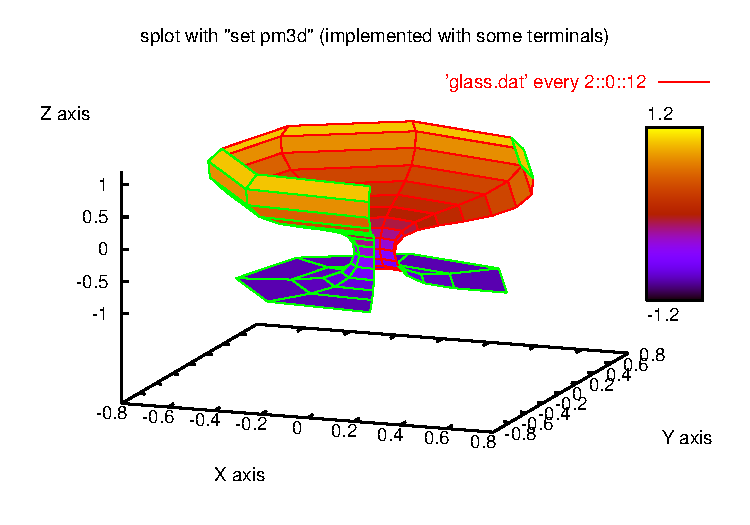
\includegraphics[width=.61\textwidth]{graph18.pdf}

\hrule \vskip 2dd

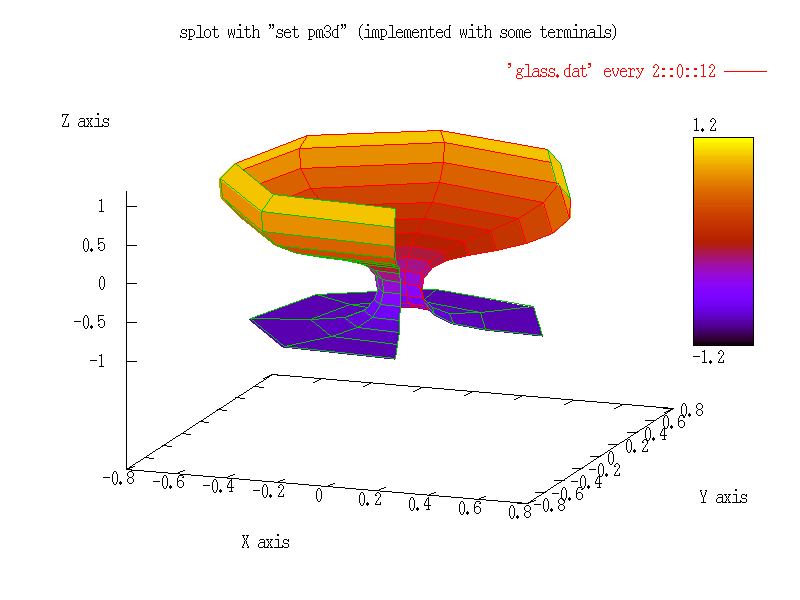
\includegraphics[width=.61\textwidth]{graph18.png}

\hrule \vskip 2dd

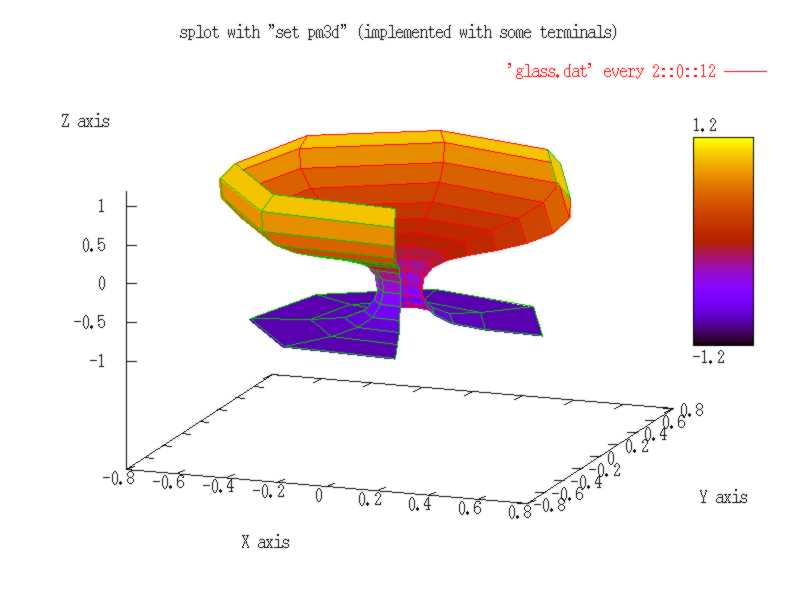
\includegraphics[width=.61\textwidth]{graph18.jpg}

}
\caption{Comparison of vector image (top) with bitmap with lossless compression (centre)
and JPEG lossy compression (bottom)}\label{vectbitfig}
\end{figure}

The top image is the vector image. It was exported as EPS\index{EPS} (Encapsulated
Post\-Script\index{Encapsulated PostScript}) and converted to PDF so that it could be
loaded by
pdf\TeX\ or by \XeTeX. The curves may look jagged on the screen, because the screen
resolution is low, but this
effect disappears when the image is printed on a quality printer.
		
The central image was exported in PNG\index{PNG} (Portable Network Graphics\index{Portable
Network
Graphics}) format. The difference in image quality is plain to see. The worse font quality
is
particularly visible. At some magnifications the axes can disappear altogether. The axes
remain
jagged even when the image is printed on a high-resolution printer, since, as mentioned
earlier,
the driver of the relevant device does not know that the pixels should all lie on the same
line and
merely recalculates the \uv{steps} at a different resolution.

Raster data take up too much memory. However, images tend to contain repeated colour
sequences and
monochromatic areas, so data can be stored more efficiently using a compression algorithm.
Compression algorithms are divided into two classes: lossless and lossy. Lossless
algorithms allow
the original data to be restored by decompression. This is impossible in principle with
lossy
algorithms.

The PNG format, used in the central image, uses a lossless compression algorithm. The
bottom image
was saved in a format that employs lossy compression --
JPEG\index{JPEG}\footnote{pronounced
\textit{jay peg}.}. This algorithm was developed by the Joint Photographic Expert
Group\index{Joint
Photographic Expert Group} for storage of colour photographs. Research has shown which
elements of
an image cannot be seen by the human eye. Such elements can thus be removed from a
photograph
without any problem. The quality is not compromised and the file size is considerably
reduced. The
quality of the image can be modified, but even with the highest image quality (lowest
compression)
the compression is always lossy. This format is called JFIF\index{JFIF} (JPEG File
Interchange
Format\index{JPEG File Interchange Format}) and the files usually have the extension
\xx\texttt{jpg}, or less often \xx\texttt{jpeg}, \xx\texttt{jff} or \xx\texttt{jfif}.

The bottom image was created at a low resolution suitable only for the screen and was
intentionally
saved at a low quality setting to make it obvious at first glance that lossy compression
leads to
blurring and the formation of colour artefacts, especially in near-monochromatic areas.

\pozor Remember that images should always be created in the format best suited to their
nature.
Charts and diagrams are always mathematical objects, which can be described using
equations known
from analytical geometry. Complicated curves are generally approximated by Bézier curves.
Such
images should therefore be created in vector format. Bitmap formats should only be used
for images
that do not have a mathematical representation. Lossless compression formats are
preferred.
Graphics formats with lossy compression should be used \textbf{solely for colour photos
and nothing
else}!

There are many myths surrounding graphics formats. One such is the belief that
EPS\index{EPS} is a
vector format. This is only partly true. EPS format is basically Post\-Script with some
restrictions. The file may contain vector or bitmap graphics or even a combination of the
two. What
matters when an image is saved in EPS format is the program that was used to create it. If
the
image was drawn using a bitmap editor such as Photoshop\index{Photoshop} or
Gimp\index{Gimp}, the
resulting EOS will also be bitmap. The same goes for PDF\index{PDF} format. Both formats
allow
lossless and lossy compression of bitmap images.

Many people mistakenly believe that there is no difference between the
(Post\-Script\index{PostScript}) and EPS\index{EPS} formats. Regrettably, this
misapprehension is
very common even among some writers of commercial software. EPS permits only a subset of
the
Post\-Script language and requires extra information before the programs can insert the
image in
the document. However, some programs create postscript files that only look like EPS. In
some cases
this doesn't matter, but often such an image cannot be inserted because it causes strange
errors
(the ensuing file gets corrupted and part of the text, or even the whole of the rest of
the
document, is lost). Sometimes an expert can repair such a file, but this can take several
hours of
investigation. Fortunately there are tools available for the job\label{poprava}. We will
touch on
these in section~\ref{oprava}.

Another myth concerns the bitmap format TIFF\index{TIFF} (Tagged Image File
Format\index{Tagged
Image File Format}; usual file extension: \xx\texttt{tif}). It is often claimed that this
format
uses lossless compression. In reality, though, the compression method can be selected when
the file
is saved. There are several lossless algorithms to choose from, and the image can even be
saved
with no compression whatsoever, but JPEG lossy compression may also be used.


\subsection{Preparing Vector Figures}\label{makevectfig} When preparing a vector figure,
it is
vital to use a graphics editor or similar program which genuinely works with vector
representation.
The figure must then be converted into a format that can be imported into the document,
i.e. EPS or
PDF. It is useful if the program is capable of writing the file in this format directly,
as is the
case, for example, with the Matlab system. If it is not, an alternative method needs to be
used.

\subsection{Virtual Printers}\label{virt} Virtual printers are an alternative solution
where the
program does not have EPS or PDF format output. However, this method is only useful if you
are
using a vector editor. A bitmap graphics editor will create a bitmap EPS or PDF even when
a virtual
printer is used.

\subsubsection{Printers with \ps{} Output}\label{virtps} Printers with \xps{} support are
available
on the market. Drivers for these printers come as a standard component of the operating
system
installation CD (Windows, Mac~OS, OS/2, eComStation). Some printers support multiple
communication
languages, such as PCL\index{PCL} and HPGL\index{HPGL}. It is inappropriate to use such
drivers in
virtual printer mode, as there are usually PJL\index{PJL} or similar commands at the start
and the
end of the file generated which enable and disable the \xps interpreter. Such commands do
more harm
than good as regards subsequent processing. Apple Writer printers are usually the best. To
create
colour images in EPS\index{EPS} format you need to install a colour printer driver, as a
monochrome
driver may convert the colours to greyscale.

Install the virtual printer as a local printer in Windows and connect it to the file
rather than to
any physical device. If the driver allows function setting, enable EPS format and select
Type~1
font conversion and insertion of fonts in the document. The standard Windows XP
installation
includes a large number of PostScript printer drivers. We have quite a good experience,
for
example, with the Apple LaserWriter Pro 600 and Lexmark Color 4079 plus PS2 printer
drivers. That
said, you will probably have to clip the EPS image (i.e. adjust the bounding box) created
by these
drivers using the method described in section \ref{oprava}.

The average CNB computer network user may not have the option of installing non-network
printers.
In such cases, it may be necessary to log in to the system as a local administrator in
order to
install a virtual local printer. After installation, this printer will be available to
other users
of the station. We recommend testing the functionality of the newly installed virtual
printer only
after logging in to the standard user account (i.e. u0xxxx).

To create a PostScript figure from a chart in MS Excel, for example, print the relevant
chart on a
virtual PostScript printer. It is a good idea to select 'Custom' under 'Printed chart
size' on the
'Chart' tab in the File/Page setup dialogue box. This will ensure that the dimensions of
the
printed chart can easily be modified in MS Excel by setting the size of the 'Chart Area'
object.
When printing, \textbf{do not tick Print to file}, but wait until the driver itself asks
you to
enter the file name.
	
\subsubsection{Printers with PDF Output}\label{virtpdf}
Adobe Acrobat\index{Acrobat}\index{Adobe Acrobat} offers a virtual printer with
PDF\index{PDF} output called PDFWriter.
	
There are also numerous PDF-generating shareware programs that can be installed as virtual
printers. Each has its own installation program. Again, where possible you should try to
enable
Type~1 font conversion and insertion of fonts in the document.

\subsection{Converting and Editing Some Graphics Formats}\label{konverzeaeditace}
When producing documents it is often necessary to convert files between EPS, PDF and WMF
formats and to modify such graphics files in other ways.

\subsubsection{Converting Figures from WMF to EPS Format}\label{wmf} Scientific
Word\index{Scientific Word} creates figures in WMF\index{WMF} (Windows
Metafile\index{Windows
Metafile}) format. To process a document in the standard \TeX{} installation you will need
to
convert the figures to EPS format. To do so you can use the shareware program
\xx\fn{wmf2eps}, an
unregistered version of which is supplied with Scientific Word version~5.5. To work
properly the
program requires installation of a virtual printer allowing print to EPS. Suitable drivers
are
supplied with the program in the \fn{PSprint} subdirectory. The installation process is
described
in the \fn{README.TXT} file in the software distribution. The program itself is very user
friendly
and intuitive.

\subsubsection{Converting Between EPS and PDF Formats}\label{epspdf}
A PS or EPS file can be converted to PDF using either Adobe
Distiller\index{Distiller}\index{Adobe Distiller} or the \xx\fn{ps2pdf} program contained
in the \xgs{} distribution (or the \xx\fn{epstopdf} program).

Conversely, to convert from PDF to EPS or PS use either the full Adobe
Acrobat\index{Acrobat}\index{Adobe Acrobat} (Save As EPS or Save As PS) or \xx\fn{pdftops}
with the
\texttt{-eps} parameter. \fn{pdftops} is part of the freely distributable \fn{xpdf}, see
\url{http://www.foolabs.com/xpdf/}.

\gs\ also offers PDF to EPS conversion, but unfortunately it rasterises the fonts at the
same time.
Such figures are not usable.

\subsubsection{Gnuplot}\label{gnuplot}\index{gnuplot} Gnuplot is a flexible, freely
distributable
program for plotting mathematical graphs. It is available for all operating systems.
Figure~\ref{vectbitfig} was created using this utility. It supports outputs in many
formats,
including EPS\index{EPS} and (in the latest version) PDF\index{PDF}.

The program offers a wide range of curve colour, dot colour and dot shape options. These
options
depend on the output format selected, and the same type of curve can even be displayed in
a
different colour in different output formats. The best way to get information is to use
the
\texttt{test} command, which will give you a test figure showing all the options that the
relevant
format has to offer. To find out what options an EPS-format output offers, use the
following
commands:

\begin{verbatim}
set term postscript eps color solid lw 2 18
set output "test.eps"
test
set output
quit
\end{verbatim}

\noindent
The test figure will be in the \fn{test.eps} file in the current directory.

\subsubsection{Corel Draw}\label{corel}\index{Corel Draw} Corel Draw is a commercial
vector image
editor. It offers export to EPS format. Bear in mind, though, that Corel Draw contains
many fonts
that are not available on other computers. When exporting to EPS, therefore, you have to
convert
such fonts into curves. In versions 8 onwards the software performs this operation
automatically.

\subsubsection{Adobe Illustrator}\label{ai}\index{Illustrator}\index{Adobe Illustrator}
Adobe
Illustrator is a commercial vector editor whose native format AI\index{AI} is based on
\ps{}. When
a file is opened in a standard text editor, it is indistinguishable from EPS at first
glance.
However, \ps\ is a programming language that has one shared feature with \TeX: it allows
definition
of user commands (using the \texttt{def} operator). The AI format contains postscript
commands, but
for these to be interpreted the defined macros contained in Adobe Illustrator are needed.
If you
insert an AI image directly into another document, everything will seem to work, but only
until you
try to print the document. On the page containing this figure, the \ps{} interpreter will
report an
\texttt{undefined} error. So don't forget to save the figure in EPS format.

\subsubsection{Repairing Corrupted EPS and PDF Files}\label{oprava}\index{EPS}\index{PDF}
In section~\ref{poprava}, on page~\pageref{poprava}, we mentioned that images in EPS and
PDF files can get corrupted. We shall now describe how to repair them.

The first common error an is an incorrect or unsuitable bounding box\index{BoundingBox}.
The
bounding box indicates the dimensions of the figure in the EPS file. According to the
specification, the entire figure must be inside the box, but there is no mention that the
box has
to be tight-fitting. If the bounding box is too large, it is not an error, but it is not
useful.
The software uses this information when inserting the figure in the document. If the
bounding box
is too large it leaves a large empty area around the figure. This is best repaired using
the freely
distributable software \xgs\ and its handy frontend \xgv. Both programs are needed. There
are
various different frontends for Linux (e.g. \xx\fn{ggv} for Gnome). Switch the orientation
of the
figure to Portrait and select the rather inappropriately named function
\texttt{PS~to~EPS}. This
does not, in fact, convert \ps\ to EPS, but just generates a tight-fitting bounding box
with the
right dimensions. In most cases the automatic setting works correctly. Use manual if
automatic
fails or if you want to remove part of the figure and you plan to use the
\hyperref[clip]{\texttt{clip}}\index{clip} parameter in the \xx\cmd{includegraphics}
macro.

\pozor \gv\ cannot determine the necessary paper size for displaying an image in EPS
format. In
addition, some programs, in particular virtual printers, do not insert the figure in the
bottom
left-hand corner. If all you see is an empty page, tick EPS~Clip\index{EPS Clip} in the
Options
menu.

The page dimensions in a PDF file can be changed using the full Adobe
Acrobat\index{Acrobat}\index{Adobe Acrobat}, which offers this function. I am not aware of
any
freely distributable alternative.

The situation is worse if the file only looks like an EPS. The simplest case is where
there are
PJL\index{PJL} or other language commands at the start and end of the file. \xgv\ can
usually cope
with these, but problems will arise when the figure is inserted. The remedy is
straightforward.
Open the file in a standard text editor and delete everything before the first occurrence
of the
characters \texttt{\%!PS} (in EPS these must be at the start of the first line) and
everything
after the text \texttt{\%\%EOF}. With a rudimentary knowledge of \ps{} you can repair
other errors.
Usually all you have to do is delete the forbidden commands, but this can be a tough task
even for
an expert. It is easier to convert the image to PDF and then back to EPS (see
\ref{epspdf}) if you
don't want to, or cannot, process the document using \pdftex.

\section{Preparing Tables}\label{tabulky} Tables are an important component of technical
papers.
However, they are only useful if they are well arranged. Producing tables is usually the
most
time-consuming part of the document preparation process. Tables are prepared using the
\xx\texttt{tabular} environment, and in this section we will present a number of
techniques that
will make it easier to typeset tables and help you achieve the desired look.

Otherwise, as with figures, tables can be inserted in the text using the \xx\texttt{table}
floating
environment. For a description of some of the more advanced techniques for working with
floating
environments, see also section \ref{plovouci}.

\subsection{Aligning Columns on a Decimal Point}\label{dcolumnuse} Decimals are often used
in
tables. The number of digits in each number of a column can differ, but it is vital that
the
numbers are aligned on the decimal point. The \xx\texttt{tabular} environment does not
offer this
option, but a solution can be found by using the \xx\fn{dcolumn} package. This package
adds column
type D to the \texttt{tabular} environment. Specification of column type D requires three
parameters: the separator used in the source text, the separator that you want to be
printed and
the maximum number of decimal places. If this last parameter is negative the decimal point
will be
in the centre of the column, which can cause the column to be too wide. The first two
parameters
are usually the same, although this need not be the case. Let's assume that we have
exported a
table from a table software package which uses decimal commas. We, however, want decimal
points. To
avoid the need to mess with the file, we make use of the option provided by the first two
parameters. An example is given in table~\ref{numtable}, the source code for which can be
seen in
figure~\ref{numtablesrc}.

\begin{table}[hbt]
\caption{Demonstration of table with decimal point alignment}\label{numtable}\vb[.5]
\centering
\setlength\extrarowheight{2pt}
\begin{tabular}{|l|D{,}{.}{2}D{,}{.}{1}|}\hline
\bfseries Jm\'eno & \multicolumn{1}{c}{\bfseries V\'y\v{s}ka [m]} &
\multicolumn{1}{c|}{\bfseries V\'aha [kg]}\\\hline
Zlatovl\'aska & 1,68 & 62,3 \\
Dlouh\'y      & 12,6 & 98,1 \\
\v{S}irok\'y  & 1,83 & 386 \\
Bystrozrak\'y & 1,74 & 74,2 \\\hline
\end{tabular}

\end{table}

\begin{figure}[hbt]
\caption{Source code for table~\ref{numtable}}\label{numtablesrc}\vb[.5]
\hrule
\verbatiminput{numtable}
\hrule
\end{figure}

The heading in column type D would not be correctly positioned. We therefore have to use
the
\xx\cmd{multicolumn} macro, in which we can change the alignment of that particular cell.
Note that
the \textbf{following} vertical line, not the preceding one, is part of the alignment
specification. The preceding line must be specified for the first column only. If, for
some (in
this case unwise) reason, the heading \textit{Jméno} should be right-aligned, we would
have to use:

\begin{verbatim}
\multicolumn{1}{|r|}{\bfseries Jm\'eno}
\end{verbatim}

The new column type definition is enabled by the fact that the \xx\fn{array} package is
implicitly loaded. This package offers users the \xx\cmd{newcolumntype} macro, which is
used to define new types. The syntax is the same as that for \cmd{newcommand}, except that
we are defining a column type, not a macro, and we cannot declare an optional parameter
with a default value. If, using the example from figure~\ref{numtablesrc}, we define a new
column type:

\begin{verbatim}
\newcolumntype{d}[1]{D{,}{.}{#1}}
\end{verbatim}

\noindent
we can write the table preamble in a plainer way:

\begin{verbatim}
\begin{tabular}{|l|d{2}d{1}|}
\end{verbatim}

In the table we have defined an extra dimension \xx\cmd{extrarowheight}, which is also
defined in
the \xx\fn{array} package. Letters with Czech diacritics are too high and there would be
almost no
space between the text and the line. The \cmd{extrarowheight} dimension register increases
the size
of the space between the text and the line above it. The parameter in square brackets of
the
\verb;\\; macro just increases the size of the space below the text.

\section{Figures and Tables as Floating Bodies}\label{plovouci} Figures and tables are
inserted in
the text using the floating environments \xx\texttt{figure} and \xx\texttt{table}, which
among
other things allow such objects to be easily numbered, described, placed and, as the case
may be,
further manipulated. Users should consult the \LaTeX\ system documentation for a
description of
basic manipulation of floating bodies. Here we describe some of the more advanced
techniques, which
will enable you to put floats exactly where you want them, to process documents with a
large number
of figures and charts and to insert rotated wide tables or charts.

\subsection{Placing Floating Bodies} The optional parameter defining where the float
should be
placed is specified in square brackets. However, \LaTeX\ treats such parameters only as
recommendations. If it is unable to execute them, it will try to place the float on a
separate
page. If even this is impossible, it will place this and all subsequent floats at the end
of the
document or chapter (in the case of a book). You should therefore specify more than one
option so
that \LaTeX\ has a choice. Stating the [h]\index{h@[h]} specifier alone usually results in
the
float being shifted to a separate page or to the end of the document. 

In some cases the float \textbf{has to be} in a specific location. You thus have to tell
\LaTeX\
that you do not mean the specifier as a recommendation but as a categorical command. The
specifier
[H]\index{H@[H]} is used for this purpose. It was originally implemented in the
\xx\fn{here}
package, but this is no longer in the standard distributions. This specifier is now
implemented in
the \xx\fn{float} package.

\pozor When [H] is used, the environment ceases to be floating. \LaTeX\ will place it in
the
desired location regardless of whether it fits in the space remaining on the page. You
should
therefore use this specifier only in the final version of the document.

\pozor This is a good place to explain the difference between the \xx\cmd{newpage} and
\xx\cmd{clearpage} / \xx\cmd{cleardoublepage} macros. The first two instruct \LaTeX\ to
start a new
page. \cmd{cleardoublepage} goes to a right-hand page\footnote{This only applies to
documents in
two-sided printing style which have the \xx\texttt{twoside} parameter specified either
explicitly
or implicitly. The \fn{cnbwp} declares it implicitly.}. In addition, the \cmd{clearpage}
and
\cmd{cleardoublepage} macros will print all the as yet unplaced floats stored in the
buffer.

\subsection{Documents with a Large Number of Figures and Tables} The floating-body
placement
algorithm is controlled by the values of several registers. The values are chosen for
normal
documents, but they may not be appropriate for technical reports with a large number of
tables and
figures. The \xx\cmd{topfraction} register defines the maximum fraction of the page that
can be
occupied by floats at the top of the page. Analogously, \xx\cmd{bottomfraction} defines
the maximum
fraction of the page for floats placed at the bottom of the page and \xx\cmd{textfraction}
is the
minimum fraction of a page that must be devoted to text. The registers are changed using
the
\xx\cmd{renewcommand} command, as they are macros. In documents with a large number of
floats they
can be set to extreme values by means of:
	
\begin{verbatim}
\renewcommand\topfraction{.99}
\renewcommand\bottomfraction{.99}
\renewcommand\textfraction{.01}
\end{verbatim}

A floating page is only created if the floats occupy at least the fraction defined in the
\xx\cmd{floatpagefraction} register. This value does not usually need changing.

\LaTeX\ also has counters, which are used to set the highest number of floats allowed.
\xx\texttt{topnumber} and \xx\texttt{bottomnumber} set the maximum number of floats at,
respectively, the top and bottom of a page, while \xx\cmd{totalnumber} limits the total
number of
floats allowed on a page. These do not usually need changing unless the document contains
a large
number of very small floats\footnote{In such case it would be worth considering grouping
them using
the \xx\fn{subfigure} package.}. The values are set using \xx\cmd{setcounter} command, for
example:

\begin{verbatim}
\setcounter{totalnumber}{17}
\end{verbatim}

\pozor The current register values can be determined in various ways. Here we will
demonstrate the use of the \TeX{} commands \xx\cmd{show} and \xx\cmd{showthe}. The former
shows the macro definition, so we will use it to determine the value of a
\textit{fraction} type register. A \textit{number} type register must be printed using
\cmd{showthe}. The following two lines will output the current values of the
\cmd{topfraction} and \cmd{topnumber} registers:

\begin{verbatim}
\show\topfraction
\showthe\value{topnumber}
\end{verbatim}

\noindent On the terminal and in the log file (we have omitted the blank lines here) we
will then
get an output like this:

\begin{verbatim}
> \topfraction=\long macro:
->.7.
l.875 \show\topfraction

> 2.
<recently read> \c@topnumber
l.876 \showthe\value{topnumber}
\end{verbatim}

\noindent We have thus determined that \cmd{topfraction} = 0.7 and \texttt{topnumber} = 2.
The full
stops at the end of the definitions are added by the \cmd{show} and \cmd{showthe}
commands.

\subsection{Wide Tables and Charts}\label{siroke} Some tables can be very wide. One way of
printing
them is to rotate them through $90^{\circ}$. This is done using the \xx\fn{rotating}
package and
the \xx\texttt{sidewaystable} environment. (Figures can be rotated analogously in the
\xx\texttt{sidewaysfigure} environment.) Unfortunately, the \fn{rotating} package rotates
tables
one way on right-hand pages and the other way on left-hand pages, which is inadmissible
from a
typographical perspective. To eliminate this problem, the package must be loaded in the
preamble in
the following way:

\begin{verbatim}
\usepackage[figuresright]{rotating}
\end{verbatim}

An example of a wide table, containing an array of random numbers calculated in
\fn{Octave} by the
$5 \times \mbox{randn}(20, 10)$ command, is given in Table~\ref{widetable}. The source
code can be
found in figure~\ref{widetablesrc}. The table will be rotated so that the left-hand margin
is
placed at the bottom margin of the typeset image (i.e. flush with the bottom margin of the
text on
the other pages). This rarely creates an aesthetic effect. A centred table looks better
and can be
obtained using the \xx\cmd{centering} command. The caption also needs to be centred by
explicitly
specifying \xx\cmd{centeredcaption} instead of \xx\cmd{caption}.

\begin{sidewaystable}[p]
\setlength{\extrarowheight}{2pt}
\newcommand\mcol[1]{\multicolumn{1}{r}{Col. #1}}
\centeredcaption{\v{S}irok\'a tabulka}\label{widetable}\bigskip\centering
\begin{tabular}{l*{10}{D{.}{.}{3}}}\hline
\bfseries \# &\mcol{1}&\mcol{2}&\mcol{3}&\mcol{4}
&\mcol{5}&\mcol{6}&\mcol{7}&\mcol{8}&\mcol{9}&\mcol{10}\\\hline
Row  1 &  -6.412 &  -2.654 &  -5.300 &   4.358 &  -6.473 &  -4.573 &   2.391 &  -0.497 &  -4.262 &  -0.341\\
Row  2 &   2.799 &  -8.109 &   5.647 &  -0.214 &   4.665 &   2.971 &  13.699 &  -5.059 &  -0.088 &   4.090\\
Row  3 &   8.427 &   5.467 &  -7.061 &  -0.347 &  -6.955 &   6.352 &  -3.955 &   7.768 &  -9.852 &   4.618\\
Row  4 &  -1.978 &  -1.226 &   1.136 &   1.733 &   3.874 &  15.072 &   4.112 &  -1.931 &   4.127 &   1.177\\
Row  5 &  10.896 &   6.859 &  -0.623 &   6.685 &  -6.378 &   2.714 &  -2.670 &   7.862 &  -2.314 &  -4.094\\
Row  6 &  -5.013 &  -2.391 &  -1.763 &  -1.499 &  -4.053 &   2.453 &   1.550 &  -3.939 &   3.366 &  -0.780\\
Row  7 &   8.644 &  -1.787 &  -5.782 &   1.244 &  -0.806 &   3.506 &   1.810 &  -3.908 &  -0.626 &  -1.933\\
Row  8 &  -4.965 &  -2.494 &   1.539 &   6.265 &   0.892 &  -2.730 &   3.311 &  -0.006 &   3.735 &   0.408\\
Row  9 &   1.237 &  -3.029 &  -0.773 &   9.400 &  -6.009 &  -0.487 &   4.281 &   4.520 &  -5.744 &  -3.628\\
Row 10 &   0.051 &  -8.717 &  -1.366 &   1.811 &  -1.599 & -10.179 &  -1.355 &   6.024 &   4.912 &   0.728\\
Row 11 &   1.894 &  -8.089 &  -6.445 &  -9.112 &  -4.753 &   2.555 &   2.751 &   0.952 &  -0.291 &  -1.523\\
Row 12 &  -3.103 &  -0.002 &   2.733 &  -9.805 &  -3.154 &  -1.985 &   4.259 &  -2.340 &  -2.236 &  -2.372\\
Row 13 &   3.729 &   1.978 &   6.627 &  -9.898 &   3.746 &  -3.595 &  -6.425 &  10.043 &   4.578 &   7.770\\
Row 14 &   9.511 &  -8.231 &   1.815 &  -5.189 &  -1.213 &   0.767 &  -2.620 &   6.613 &  -1.119 &  -3.838\\
Row 15 &  -0.699 & -10.599 &   5.787 & -11.333 &  -4.810 &   2.769 &   0.255 &  -6.831 &  -1.643 &  -2.870\\
Row 16 &   7.190 &  -2.291 &   7.532 &   2.650 &  -5.878 &  -4.859 &   7.792 &  -1.337 &  -5.075 &  -7.241\\
Row 17 &  -5.918 &   0.987 &   5.037 &  -0.556 &  -2.653 &  -7.008 &   3.491 &  -1.028 &   0.573 &   4.620\\
Row 18 &  -3.957 &  -4.265 &   1.325 &   3.102 &  -5.731 &  -3.944 &  -6.565 &   5.178 &   2.477 &  -1.948\\
Row 19 &  -1.228 &  -0.170 &  -3.048 &  -2.966 &   9.791 &   9.006 &   9.186 &  -2.971 &   8.657 &  -2.838\\
Row 20 &  -2.340 &  -4.932 &  -3.904 &   4.164 &  -5.838 &  -7.320 &   1.451 &   4.955 &   7.439 &  -4.407\\
\hline
\end{tabular}
\end{sidewaystable}


\begin{sidewaysfigure}[p]
\caption{Source code for table \ref{widetable}}\vb[.5]\label{widetablesrc}
\small
\hrule
\verbatiminput{widematrix}
\end{sidewaysfigure}

Table centering need not always be desirable. The page setup can be altered by shifting
the table.
Prepare the page without centering the table and print it out or display it in \xgv\ (this
program
allows you to make measurements). Let's assume that you want to shift the table 27\,mm
towards the
top margin of the page. This means that you have to widen the left-hand margin of the
floating
environment by the same amount. This is done by specifying the following at the beginning
of the
environment:

\begin{verbatim}
\begin{sidewaystable}[p]% beginning of rotated table
\setlength{\leftskip}{27mm}
\end{verbatim}

\noindent This command will shift the table and the standard caption, although it will not
work
correctly when \xx\cmd{centeredcaption} is used.

\pozor Note that the \xx\cmd{label} command must be written inside the floating
environment to
which it relates and after the \cmd{caption} macro or the alternative thereto defined in
the
\fn{cnbwp} class. If it is written outside this environment or before the \cmd{caption}
macro, it
will relate to the \cmd{section} or \cmd{subsection} in which it occurs.

\section{Generating the Final Document in PDF Format}\label{latex2pdf} Czech National Bank
Working
Papers are published in PDF\index{PDF} format. We will therefore focus on the most common
methods
of generating a PDF file from a text written in \LaTeX.

The first option is to generate the PDF\index{PDF} document directly, using \xpdftex. If
you
cannot, or do not want to, use this, you can convert the DVI output file to \xps\ using
\xx\fn{dvips}. The postscript file can then be converted to PDF using a software package
(commercial and freely distributable products are both available). See also section
\ref{konverzeaeditace}.

Scientific Word\index{Scientific Word} does not contain \xx\fn{dvips}. The PDF can thus
only be
generated using a virtual printer. Adobe Distiller tends to produce better results than
PDFWriter\index{PDFWriter}, although for short documents the difference is not usually
significant.
As Scientific Word generates a \LaTeX{} file, this file can also be transferred onto a
computer
with the full \TeX{} installation and the PDF can be generated in the usual way using
\xpdftex or
via \xps\ and conversion to PDF. Figures in WMF\index{WMF} format have to be converted to
EPS\index{EPS} using \xx\fn{wmf2eps}, as mentioned in section~\ref{wmf}.

Another option is to generate the PDF from the DVI using \xx\fn{dvipdfm}, which is part of
the MikTeX distribution, for example.

To print the document from PDF you may need to adjust the margin settings. The drivers of
some
physical printers ignore the margins set in the file and shift the text on the paper.
Adjusting
margin settings is described in section /ref{preambule}.

\section{Submitting Your Document for Editing and Publication}\label{publish} When
preparing your
document for submission, you should bear in mind that the editor is not necessarily a
\LaTeX expert
and might not even have any \TeX{} distribution installed. You should therefore submit a
file that
can be printed out using standard, easy-to-install software, hence preferably in PDF
format or, as
a last resort, as a \ps file.
	
By agreement with our editor, CNB research publications are currently submitted for
editing in two
formats: PDF and the (\LaTeX) source text saved as an MS Word document. The editor opens
the source
text in MS Word and edits it with Track Changes enabled, using the PDF version for
guidance.

The CNB editor has been told to emend linguistic phenomena only. He does not alter
formatting
commands that start with a backslash, including their arguments in curly or square
brackets. In
other words, he only corrects the words he sees in the printed version. For example, he
also leaves
apostrophes and hyphens unchanged. However, it is the author's responsibility to further
process
the edited text and either accept or reject each change. We do not recommend accepting all
the
changes in one step. Finally, the edited file is saved as plain text with the extension
\texttt{.tex} and can be processed using the \LaTeX system.

The main document can load other files using the \cmd{input} or \cmd{include} commands.
The name of
the file to be loaded is written in a parameter of this macro. The \texttt{.tex} extension
need not
be given. However, keep these commands to a minimum when writing documents for CNB WP
purposes.
Excessive use reduces clarity and leads to complications during editing.

Do not use letters with diacritics. There are too many codings for Czech and Slovak, and
different
\TeX{} distributions treat these codings differently. You should assume that your document
will be
worked on by a somewhat informed layman who may not be able to cope with recoding. So,
always write
diacritics using \TeX sequences.

All the files needed for typesetting the documents should be in the same directory or (in
exceptional cases) in subdirectories of the directory containing the main document. The
command

\begin{verbatim}
\includegraphics{d:/projects/figures/image1.eps}
\end{verbatim}

\noindent

is bad for three reasons:

\begin{enumerate}
\item The author of the document might forget that a vital file is in a different
directory and will forget to bundle it.
\item The person processing the document might have different disk partitioning and the
command will return a File Not Found message.
\item For security reasons, some \TeX{} installations do not permit absolute paths or
access to the parent directory.
\end{enumerate}

Unix users should resist the temptation to use symbolic links in such cases. For one
thing, it can
easily occur that only the symbolic links, and not the files, are bundled with the
document. In
addition, the document has to be processable on a file system which does not support
symbolic
links. If you use subdirectories, enter the names relatively, for example:

\begin{verbatim}
\includegraphics{figures/image1.eps}
\end{verbatim}

\noindent Always consider, however, whether it is really necessary to create
subdirectories. For
the uninitiated, it is usually clearer if all related files are saved in the same
directory.

\pozor Do not use file names that contain spaces and/or diacritics. The \TeX book states
that a
space terminates a file name. Given the popularity of spaces with Microsoft, there are
distributions around which can cope with this. It is, however, a \textbf{very non-standard
distribution} and may not even work on the same operating system with a different \TeX{}
distribution. Directory and file names containing diacritics are an even worse problem.
Whether
they work depends on too many factors -- not only the \TeX{} distribution, but also the
locales
settings in the operating system. Such names should be avoided, as they are highly likely
to cause
problems.

All the necessary files must be packed into a single archive with a directory structure.
ZIP is the
best format. Add a short explanatory text in a file named \fn{readme.txt}, especially if
the
document comprises multiple files.

\TeX\ was created at a time when texts were entered into computers on punch cards.
Consequently, it
does not matter how the text is divided into lines and how many spaces there are between
words. The
important thing is to leave a blank line between paragraphs.

As an interesting alternative a PDF file may directly be used for carrying out the proof.
Commenting must be enabled by full version of Adobe Acrobat\index{Acrobat}\index{Adobe
Acrobat} and the proof can ten be done by Acrobat Reader\index{Acrobat Reader}.

\section{Sample Files}\label{vzor} This manual includes a number of sample files. The main
document
template is in the file \xx\fn{cnbpaper.tex} and the entire document has been converted
into PDF
format (\xx\fn{cnbpaper.pdf}) using pdf\LaTeX{}. However, the file can also be processed
using the
standard \LaTeX and the \fn{dvips} program.

Some examples are saved in separate files, partly to ensure that they are consistent with
this
manual, and partly so that users do not have to work with a lengthy sample document when
writing
their texts.

Table~\ref{numtable}, demonstrating decimal point alignment, is located in
\xx\fn{numtable.tex}.
Neither the \cmd{caption} command nor a floating environment is specified in this file.
These
commands can be found in the main document template.

The wide table~\ref{widetable} can be found in \xx\fn{widematrix.tex}. In this case the
file also contains environment definition commands.

The files \xx\fn{graf18.eps} and \xx\fn{graf18.pdf} are the vector charts from
figure~\ref{vectbitfig}. The template uses the \xx\fn{ifpdf} package to determine whether
pdf\LaTeX
is being used, and the file will accordingly be loaded in the correct format. If
\fn{ifpdf} is not
contained in the distribution, it will be assumed that pdf\LaTeX\ is unavailable.

The file \xx\fn{biblio.tex} contains a list of references written using the macros from
section~\ref{makra}. The full list is given in the \hyperref[priloha]{Appendix}.

The file \xx\fn{cnbsample.bib} contains the list of references for use with \BibTeX. It
was also used to generate the above mentioned file \fn{biblio.tex}.

If you intend to use \fn{cnbpaper.tex} as the template for your document, think about
which
packages you really need. Delete any unnecessary \cmd{usepackage} commands. You may need
some
additional packages, such as \xx\fn{amsmath}.

\section{Changes, Version 2013.12}
The following changes were made in December, 2013:
\begin{enumerate}
\item Switches 11pt and 12pt for changing the font size were removed.
\item The syntax of the \cmd{author} macro was changed.
\item Macros \xx\cmd{shortauthor} and \xx\cmd{shorttitle} were removed.
\item Usage of the \cmd{acknowledge} macro was changed.
\item The \texttt{abstrakt} environment for entering the Czech abstract was added.
\item The \fn{babel} package is loaded in order to activat the Czech hyphenation rules in
the \fn{abstrakt} environment.
\item Captions formatting modified to comply with the new requirements.
\item New macros \cmd{Note} and \cmd{Source} were implemented.
\item Formatting of the author names in the \fn{abbrvcnb} style was modified.
\item The \fn{times} package replaced with the \fn{mathptmx}.
\item The manual was updated.
\end{enumerate}

\appendix
\section{Appendix}\label{priloha}
The annex gives examples of all types of works written using the macros from
section~\ref{makra} and the subsections thereof. You will not normally use the \;note\
field.

The entire set of examples is also available in \xx\fn{biblio.tex}.

{\small
\verbatiminput{biblio}}

\printindex
\end{document}
